\setAuthor{Jaan Kalda}
\setRound{lõppvoor}
\setYear{2014}
\setNumber{G 5}
\setDifficulty{6}
\setTopic{Kinemaatika}

\prob{Kammid}
\begin{wrapfigure}{r}{0.6\textwidth}%
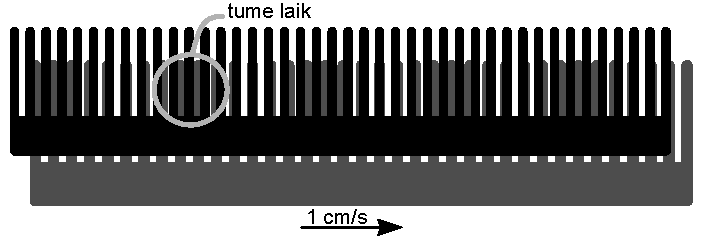
\includegraphics[width=1\linewidth]{2014-v3g-05-kammid}
\end{wrapfigure}

Kaks kammi on asetatud üksteise taha nii, nagu näidatud joonisel. Halli kammi liigutatakse kiirusega $v=\SI 1{cm/s}$ ning musta kammi hoitakse paigal. Millise kiirusega ja millises suunas liiguvad tumedad laigud?

\hint
Kui hall kamm liigub ühe pii võrra, on uus pilt identne esialgsega ning järelikult on tume laik liikunud ühe \enquote{lainepikkuse} võrra.

\solu
Kui hall kamm liigub ühe pii võrra, on uus pilt identne esialgsega ning järelikult on tume laik liikunud ühe \enquote{lainepikkuse} võrra. 
Ühe laikude \enquote{lainepikkuse} kohta tuleb 7 halli kammi piide \enquote{lainepikkust}, seega liiguvad hallid laigud 7 korda kiiremini kui hall kamm: $v=\SI 7{cm/s}$.

\probeng{Combs}
Two combs are placed behind each other as in the figure. The grey comb is moved with a speed $v=\SI 1{cm/s}$ and the black comb is held still.  With what speed and to what direction are the dark spots moving?
\begin{center}
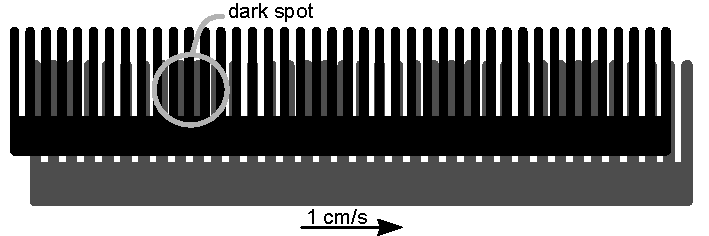
\includegraphics[width=0.6\textwidth]{2014-v3g-05-kammid_ing}
\end{center}

\hinteng
If the grey comb moves by one teeth then the new picture is identical with the initial one and thus the dark spot has moved by one “wavelength”.

\solueng
If the grey comb moves by one teeth then the new figure is identical to the initial one and therefore the dark spot has moved by one “wavelength”. For one “wavelength” of the spots there are 7 “wavelengths” of the grey comb’s teeth, therefore the grey spots move 7 times faster than the grey comb: $v=\SI 7{cm/s}$.
\probend